\section{Design Flow}
\label{sec:design_flow}

Design entry is done mostly with Verilog or Wokwi~\cite{wokwi}.
Wokwi is a web based schematic based editor that is an easy way to get started for people with no prior hardware description language (HDL) experience.
The TinyTapeout website~\cite{tinytapeout} includes a basic getting started guide for drawing circuits with Wokwi available in English and Spanish.

The design flow consists of templating a GitHub~\cite{github} repository, adding a design, waiting for the tests and binary layout files (GDS~\cite{gds}) generation to complete, then submitting to a quarterly shuttle.

The GitHub templates\cite{verilogtemplate} make use of GitHub Actions\cite{githubactions} - an automatic continuous integration system that is triggered every time the repository is updated.

There are 4 main jobs:

\begin{enumerate}
	\item GDS - installs OpenLane\cite{openlane} and the Sky130\cite{skywaterpdk} PDK, builds the GDS and generates a summary of the design (Fig.~\ref{fig:summary_table_GDS_job}). The summary includes utilization, standard cells used, a 2D render (Fig.~\ref{fig:render_cells_in_use}) and an interactive 3D viewer (Fig.~\ref{fig:interactive_3D_viewer}).
This job can also optionally run a gate-level verification.
	\item Verification - installs the YosysHQ open source CAD suite which includes many common electronic design automation (EDA) tools.
Then iVerilog\cite{iverilog} and cocotb\cite{cocotb} are used to run any testbenches included.
	\item Documentation - generates a preview of the documentation.
	\item Precheck - a number of tests are run to make sure that the design doesn’t cause design rule check (DRC) errors after integration into the chip.
\end{enumerate}

Successful GDS, Documentation, and Precheck jobs are required to submit to a shuttle.
Verification is optional but highly encouraged. Wokwi designs can make use of an integrated truth table testing system\cite{automatedtesting}.

While the process can be done entirely in the browser, it’s also possible to install a local copy of the tools\cite{localinstall}, which can help to reduce iteration time, especially for tests and verification.

\begin{figure}[htp]
\centering
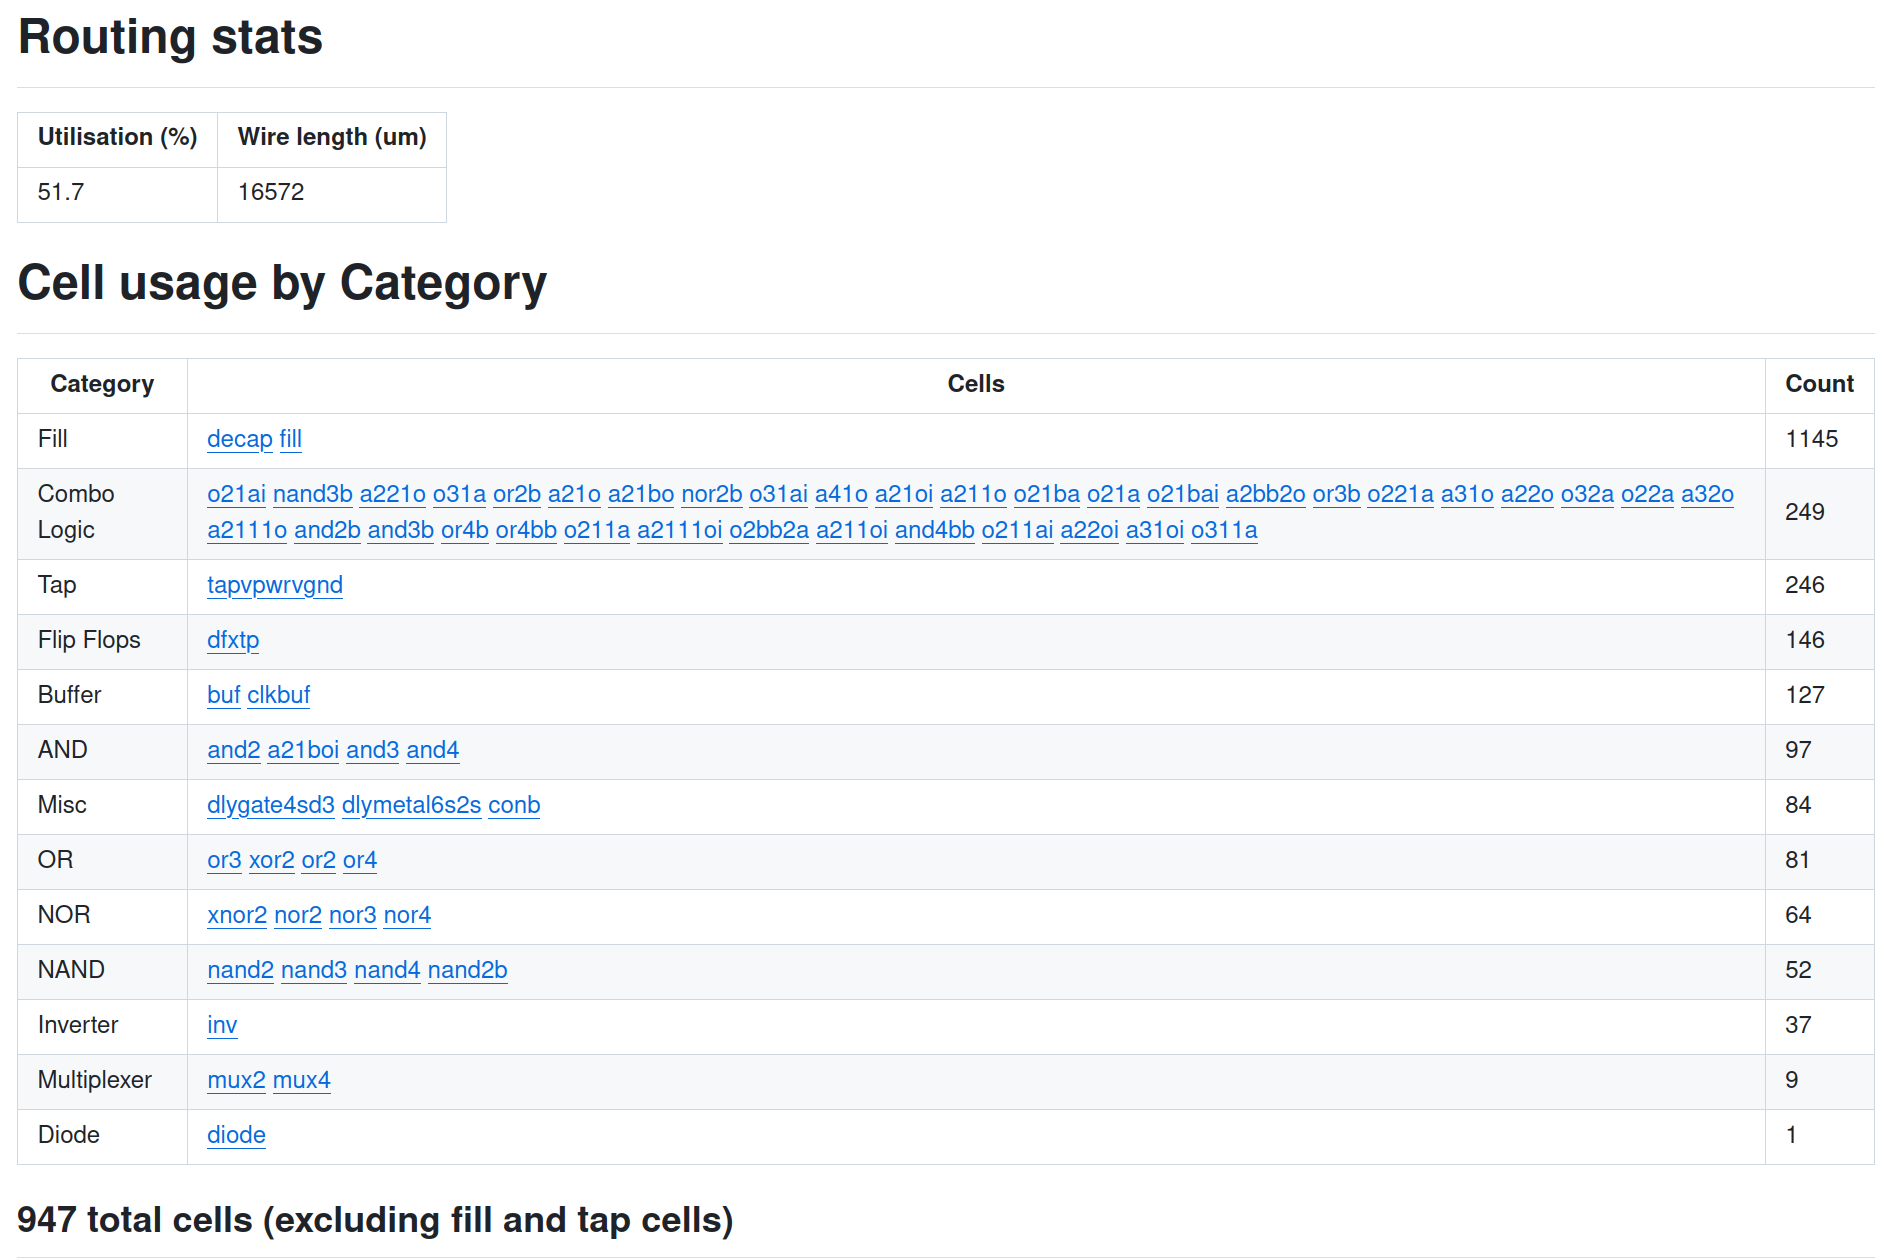
\includegraphics[width=\columnwidth]{./Figs/gh action cell stats.png}
\caption{The summary table of the GDS job.}
\label{fig:summary_table_GDS_job}
\end{figure}

\begin{figure}[htp]
\centering
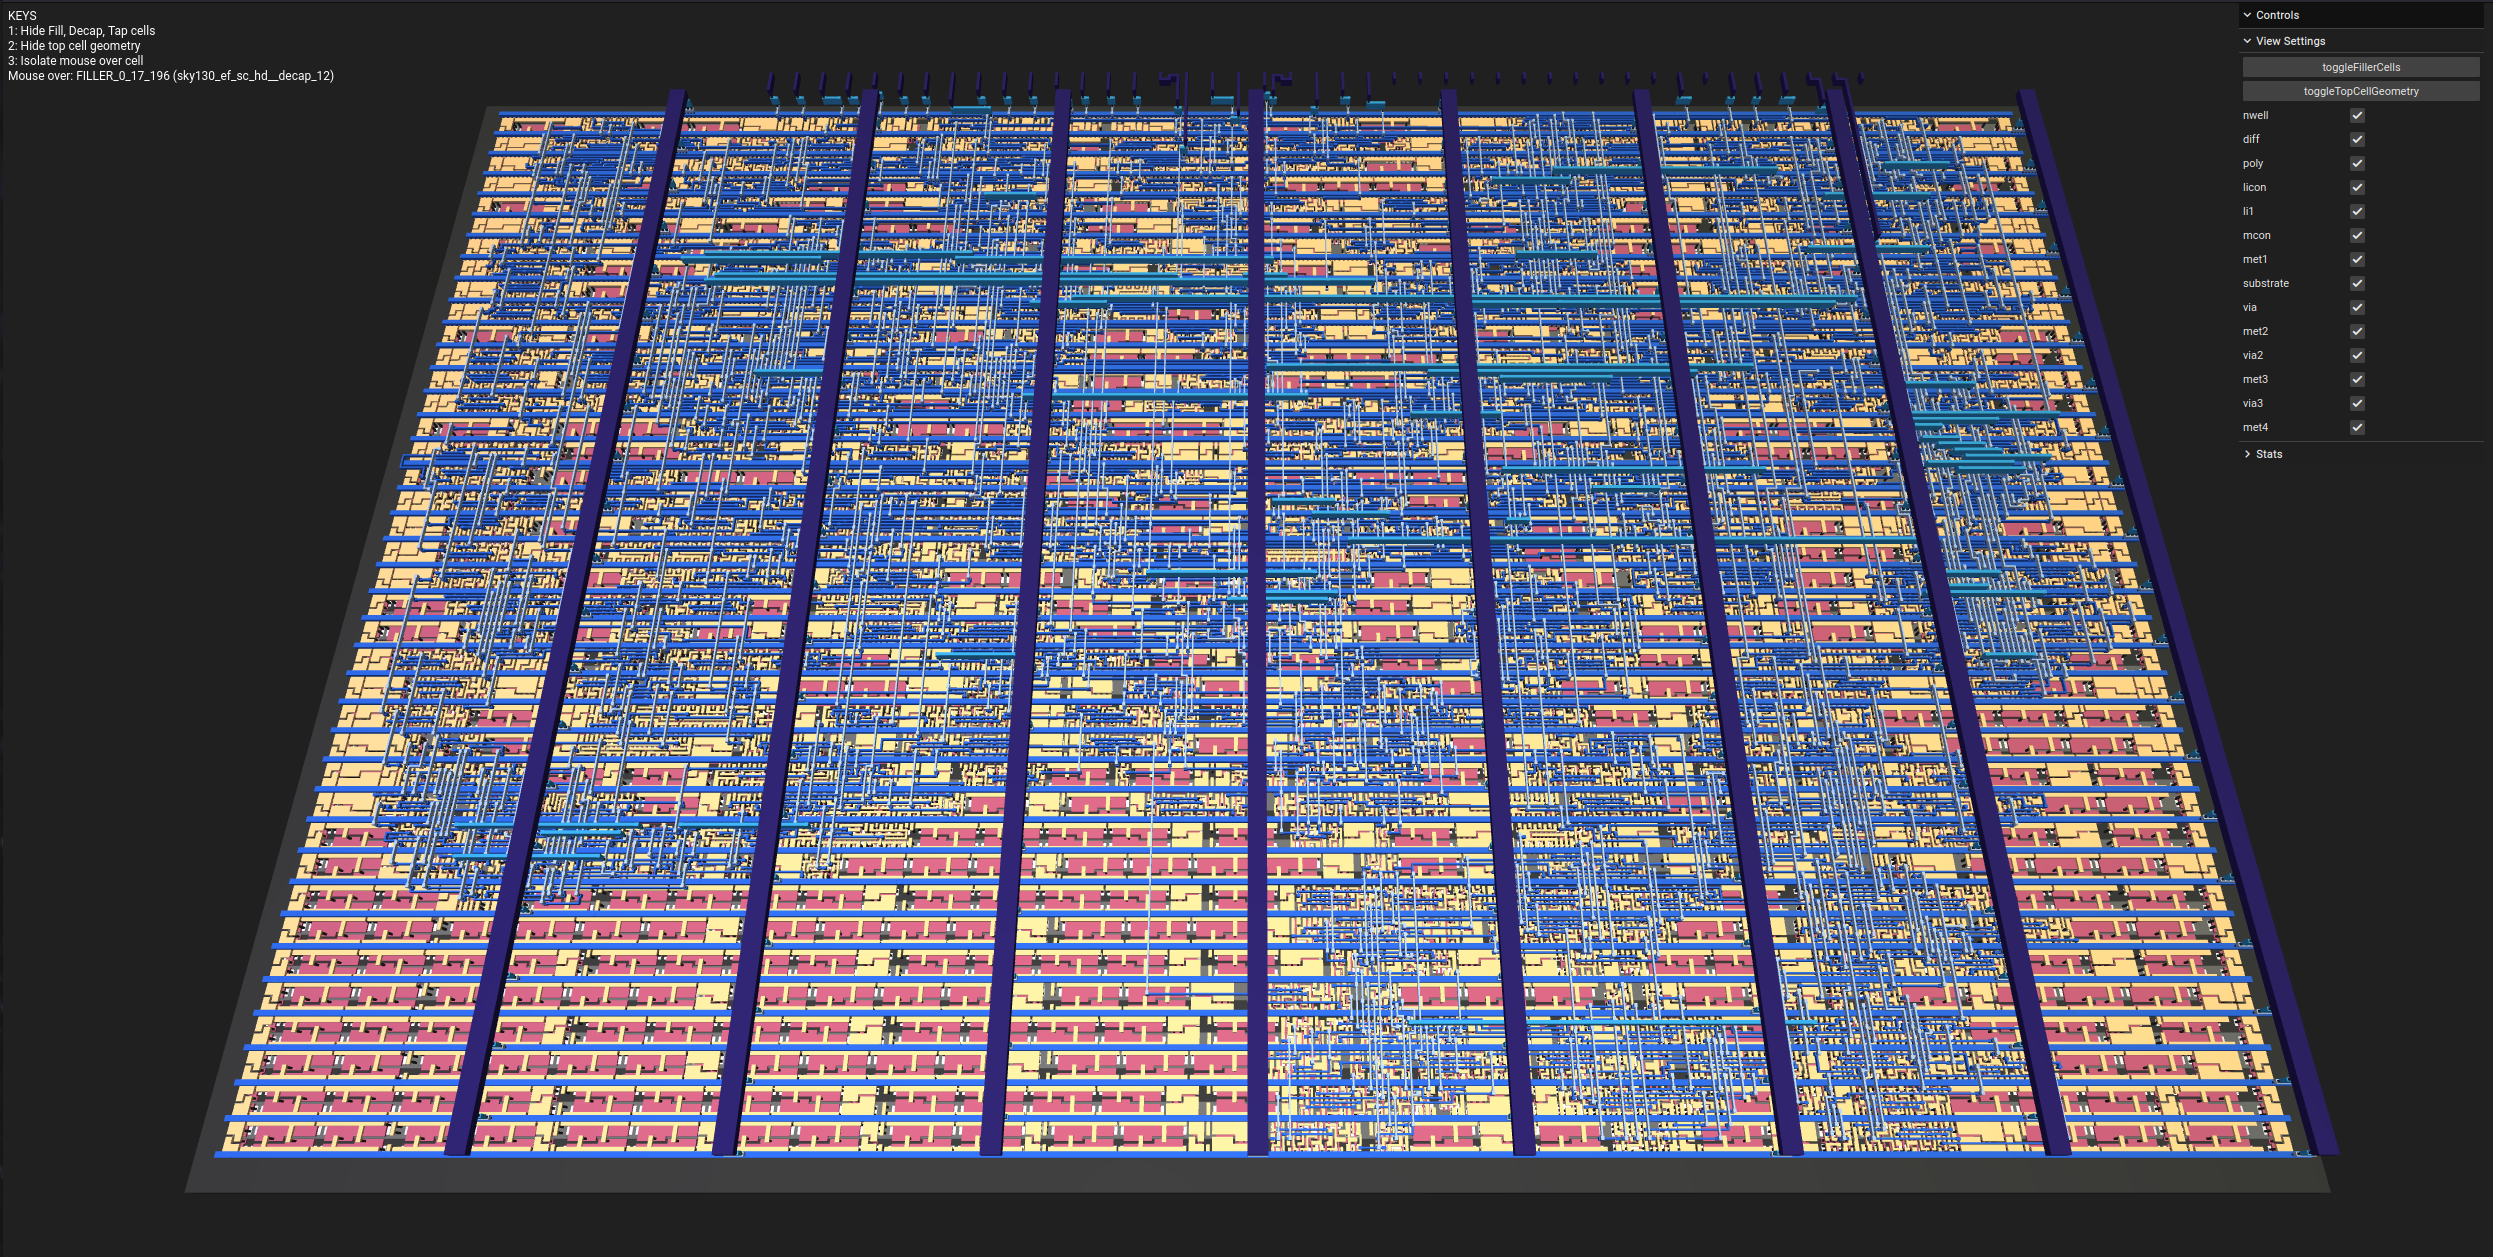
\includegraphics[width=\columnwidth]{./Figs/gh action gds 3d view.png}
\caption{The interactive 3D viewer.}
\label{fig:interactive_3D_viewer}
\end{figure}
